% Copyright 2003 by Till Tantau <tantau@cs.tu-berlin.de>.
%
% This program can be redistributed and/or modified under the terms
% of the LaTeX Project Public License Distributed from CTAN
% archives in directory macros/latex/base/lppl.txt.


\section{Declaring and Using Shadings}

\label{section-shadings}

\subsection{Overview}

A shading is an area in which the color changes smoothly between different
colors. Note also that |ghostview| may do a poor job at displaying
shadings when doing anti-aliasing. 

Similarly to an image, a shading must first be declared before it can
be used. Also similarly to an image, a shading is put into a
\TeX-box. Hence, in order to include a shading in a |{pgfpicture}|,
you have to use |\pgftext| around it.

There are three kinds of shadings: horizontal, vertical, and radial
shadings. However, you can rotate and clip shadings like any other
graphics object, which allows you to create more complicated
shadings. Horizontal shadings could be created by rotating a vertical
shading by 90 degrees, but explicit commands for creating both
horizontal and vertical shadings are included for convenience.

Once you have declared a shading, you can insert it into text using
the command |\pgfuseshading|. This command cannot be used directly in
a |{pgfpicture}|, you have to put a |\pgftext| around it. The second
command for using shadings, |\pgfshadepath|, on the other hand, can
only be used  inside |{pgfpicture}| environments. It will ``fill'' the
current path with the shading.

A horizontal shading is a horizontal bar of a certain height whose
color changes smoothly. You must at least specify the colors at the
left and at the right end of the bar, but you can also add color
specifications for points inbetween. For example, suppose you
which to create a bar that is red at the left end, green in the
middle, and blue at the end. Suppose you would like the bar to be 4cm
long. This could be specified as follows:
\begin{codeexample}[code only]
rgb(0cm)=(1,0,0); rgb(2cm)=(0,1,0); rgb(4cm)=(0,0,1)
\end{codeexample}
This line means that at 0cm (the left end) of the bar, the color
should be red, which has red-green-blue (rgb) components (1,0,0). At
2cm, the bar should be green, and at 4cm it should be blue.
Instead of |rgb|, you can currently also specify |gray| as
color model, in which case only one value is needed, or |color|,
in which case you must provide the name of a color in round
brackets. In a color specification the individual specifications must
be separated using a semicolon, which may be followed by a whitespace
(like a space or a newline). Individual specifications must be given
in increasing order. 

\subsection{Declaring Shadings}

\begin{command}{\pgfdeclarehorizontalshading\oarg{color list}\marg{shading
      name}\marg{shading height}\marg{color specification}}
  Declares a horizontal shading named \meta{shading name} of the specified
  \meta{height} with the specified colors. The length of the bar is
  automatically deduced from the maximum specification.

\begin{codeexample}[]
\pgfdeclarehorizontalshading{myshading}
  {1cm}{rgb(0cm)=(1,0,0); color(2cm)=(green); color(4cm)=(blue)}
\pgfuseshading{myshading}
\end{codeexample}

  The effect of the \meta{color list}, which is a
  comma-separated list of colors, is the following: Normally, when
  this list is empty, once a shading is declared it becomes
  ``frozen.'' This means that even if you change a color that was used
  in the declaration of the shading later on, the shading will not
  change. By specifying a \meta{color list} you can specify
  that the shading should be recalculated whenever one of the colors
  listed in the list changes (this includes effects like color
  mixins). Thus, when you specify a \meta{color list},
  whenever the shading is used, \pgfname\ first converts the colors in the
  list to \textsc{rgb} triples using the current values of the
  colors and taking any mixins and blendings into account. If the
  resulting \textsc{rgb} triples have not yet been   used, a new
  shading is internally created and used. Note that if the 
  option \meta{color list} is used, then no shading is created until
  the first use of |\pgfuseshading|. In particular, the colors
  mentioned in the shading need not be defined when the declaration is
  given.

  When a shading is recalculated because of a change in the
  colors mentioned in \meta{color list}, the complete shading
  is recalculated. Thus even colors not mentioned in the list will be
  used with their current values, not with the values they had upon
  declaration.
  
\begin{codeexample}[]
\pgfdeclarehorizontalshading[mycolor]{myshading}
  {1cm}{rgb(0cm)=(1,0,0); color(2cm)=(mycolor)}
\colorlet{mycolor}{green}
\pgfuseshading{myshading}
\colorlet{mycolor}{blue}
\pgfuseshading{myshading}
\end{codeexample}
\end{command}


\begin{command}{\pgfdeclareverticalshading\oarg{color list}\marg{shading
      name}\marg{shading width}\marg{color specification}}
   Declares a vertical shading named \meta{shading name} of the
   specified \meta{width}. The height of the bar is automatically
   deduced from the maximum specification. The effect of \opt{color
     list} is the same as for horizontal shadings.

\begin{codeexample}[]
\pgfdeclareverticalshading{myshading2}
  {4cm}{rgb(0cm)=(1,0,0); rgb(1.5cm)=(0,1,0); rgb(2cm)=(0,0,1)}
\pgfuseshading{myshading2}
\end{codeexample}
\end{command}


\begin{command}{\pgfdeclareradialshading\oarg{color list}\marg{shading
      name}\marg{center point}\marg{color specification}}
  Declares an radial shading. A radial shading is a circle whose inner
  color changes as specified by the color specification. Assuming that
  the center of the shading is at the origin, the color of the center
  will be the color specified for 0cm and the color of the border of
  the circle will be the color for the maximum specification. The
  radius of the circle will be the maximum specification. If the
  center coordinate is not at the origin, the whole shading inside the
  circle (whose size remains exactly the same) will be distorted such
  that the given center now has the color specified for 0cm. The
  effect of \opt{color list} is the same as for horizontal shadings.

\begin{codeexample}[]  
\pgfdeclareradialshading{sphere}{\pgfpoint{0.5cm}{0.5cm}}%
  {rgb(0cm)=(0.9,0,0);
   rgb(0.7cm)=(0.7,0,0);
   rgb(1cm)=(0.5,0,0);
   rgb(1.05cm)=(1,1,1)}
\pgfuseshading{sphere}
\end{codeexample}
\end{command}


\begin{command}{\pgfaliasshading\marg{new shading name}\marg{existing shading name}}
  The \meta{existing shading name} is ``cloned'' and the shading
  \meta{new shading name} can now be used whenever original shading
  is used. This command is mainly useful for creating aliases for
  environments that use alternate extensions.
  \example \verb/\pgfaliasshading{shading!30}{shading!25}/
\end{command}


\subsection{Using Shadings}
\label{section-shading-a-path}

\begin{command}{\pgfuseshading\marg{shading name}}
  Inserts a previously declared shading into the text. If you wish to
  use it in a |pgfpicture| environment, you should put a |\pgfbox|
  around it. Like |\pgfuseimage|, alternate extensions are tried
  before the actual shading is used.

\begin{codeexample}[]
\begin{pgfpicture}
  \pgfdeclareverticalshading{shading}
    {20pt}{color(0pt)=(red); color(20pt)=(blue)}
  \pgftext[at=\pgfpoint{1cm}{0cm}]  {\pgfuseshading{shading}}
  \pgftext[at=\pgfpoint{2cm}{0.5cm}]{\pgfuseshading{shading}}
\end{pgfpicture}
\end{codeexample}
\end{command}

\begin{command}{\pgfshadepath\marg{shading name}\marg{angle}}
  This command must be used inside a |{pgfpicture}| environment. The
  effect is a bit complex, so let us go over it step by step.

  First, \pgfname\ will setup a local scope.

  Second, it uses the current path to clip everything inside this
  scope. However, the current path is once more available after the
  scope, so it can be used, for example, to stroke it.

  Now, the \meta{shading name} should be a shading whose width and
  height are 100\,bp, that is, 100 big points. \pgfname\ has a look at
  the bounding box of the current path. This bounding box is computed
  automatically when a path is computed; however, it can sometimes be
  (quite a bit) too large, especially when complicated curves are
  involved. 

  Inside the scope, the lowlevel transformation matrix is modified.
  The center of the shading is translated (moved) such that it lies on
  the center of the bounding box of the path. The lowlevel coordinate
  system is also scaled such that the shading ``covers'' the shading (the 
  details are a bit more complex, see below). Finally, the coordinate
  system is rotated by \meta{angle}.

  After everything has been set up, the shading is inserted. Due to
  the transformations and clippings, the effect will be that  the
  shading seems to ``fill'' the path.

  If both the path and the shadings were always be rectangles and if
  rotation were never involved, it would be easy to scale shadings
  such they always cover the path. However, when a vertical shading is
  rotated, must must obviously ``magnify'' the shading so that it
  still covers the path. Things get worse when the path is not a
  rectangle itself.

  For these reasons, things work slightly differently ``in reality.''
  The shading is scaled (more precisely, the coordinate system is
  scaled, but never mind the difference) and translated such that the
  the point $(50\mathrm{bp},50\mathrm{bp})$, which is the middle of
  the shading, is at the middle of the path and such that the the
  point $(25\mathrm{bp},25\mathrm{bp})$ is at the lower left corner of
  the path and that  $(75\mathrm{bp},75\mathrm{bp})$  is at upper
  right corner.

  In other words, only the center quarter of the shading will actually
  ``survive the clipping'' if the path is a rectangle. If it is not a
  rectangle, but, say, a circle, even less is seen of the
  shading. Here is an example that demonstrates this effect:

\begin{codeexample}[]
\pgfdeclareverticalshading{shading}{100bp}    
 {color(0bp)=(red); color(25bp)=(green);  color(75bp)=(blue);  color(100bp)=(black)}
\pgfuseshading{shading}
\hskip 1cm
\begin{pgfpicture}
  \pgfpathrectangle{\pgfpointorigin}{\pgfpoint{2cm}{1cm}}
  \pgfshadepath{shading}{0}
  \pgfusepath{stroke}
  \pgfpathrectangle{\pgfpoint{3cm}{0cm}}{\pgfpoint{1cm}{2cm}}
  \pgfshadepath{shading}{0}
  \pgfusepath{stroke}
  \pgfpathrectangle{\pgfpoint{5cm}{0cm}}{\pgfpoint{2cm}{2cm}}
  \pgfshadepath{shading}{45}
  \pgfusepath{stroke}
  \pgfpathcircle{\pgfpoint{9cm}{1cm}}{1cm}
  \pgfshadepath{shading}{45}
  \pgfusepath{stroke}
\end{pgfpicture}
\end{codeexample}

  As can be seen above in the last case, the ``hidden'' part of the
  shading actually \emph{can} become visible if the shading is
  rotated. The reason is that it is scaled as if no rotation took
  place, then the rotation is done.

  The following graphics show which part of the shading are actually
  shown: 

\begin{codeexample}[]
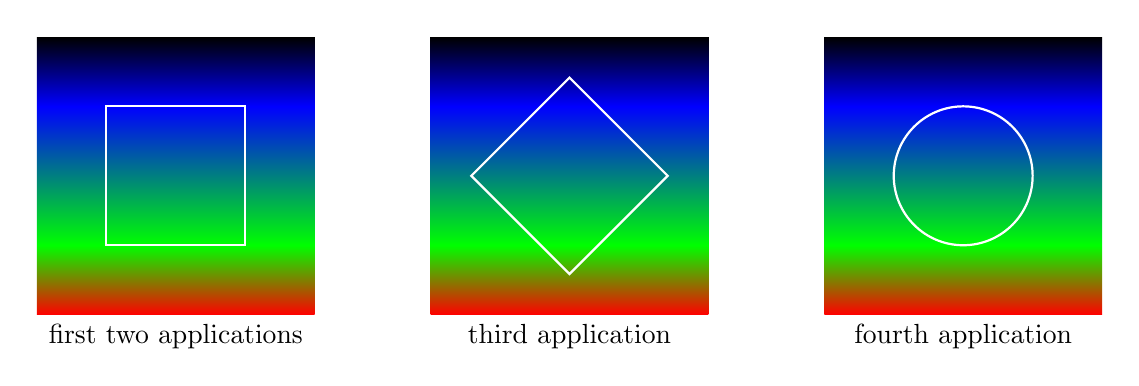
\begin{tikzpicture}
  \draw (50bp,50bp) node {\pgfuseshading{shading}};
  \draw[white,thick] (25bp,25bp) rectangle (75bp,75bp);
  \draw (50bp,0bp) node[below] {first two applications};

  \begin{scope}[xshift=5cm]
    \draw (50bp,50bp) node{\pgfuseshading{shading}};
    \draw[rotate around={45:(50bp,50bp)},white,thick] (25bp,25bp) rectangle (75bp,75bp);
    \draw (50bp,0bp) node[below] {third application};
  \end{scope}

  \begin{scope}[xshift=10cm]
    \draw (50bp,50bp) node{\pgfuseshading{shading}};
    \draw[white,thick] (50bp,50bp) circle (25bp);
    \draw (50bp,0bp) node[below] {fourth application};
  \end{scope}
\end{tikzpicture}
\end{codeexample}
  
  An advantage of this approach is that when you rotate a radial
  shading, no distortion is introduced:

\begin{codeexample}[]
\pgfdeclareradialshading{ballshading}{\pgfpoint{-10bp}{10bp}}
 {color(0bp)=(red!15!white); color(9bp)=(red!75!white);
 color(18bp)=(red!70!black); color(25bp)=(red!50!black); color(50bp)=(black)}
\pgfuseshading{ballshading}
\hskip 1cm
\begin{pgfpicture}
  \pgfpathrectangle{\pgfpointorigin}{\pgfpoint{1cm}{1cm}}
  \pgfshadepath{ballshading}{0}
  \pgfusepath{}
  \pgfpathcircle{\pgfpoint{3cm}{0cm}}{1cm}
  \pgfshadepath{ballshading}{0}
  \pgfusepath{}
  \pgfpathcircle{\pgfpoint{6cm}{0cm}}{1cm}
  \pgfshadepath{ballshading}{45}
  \pgfusepath{}
\end{pgfpicture}
\end{codeexample}

  If you specify a rotation of $90^\circ$
  and if the path is not a square, but an elongated rectangle,  the
  ``desired'' effect results: The shading will exactly vary between
  the colors at the 25bp and 75bp boundaries. Here is an example:
  
\begin{codeexample}[]
\begin{pgfpicture}
  \pgfpathrectangle{\pgfpointorigin}{\pgfpoint{2cm}{1cm}}
  \pgfshadepath{shading}{0}
  \pgfusepath{stroke}
  \pgfpathrectangle{\pgfpoint{3cm}{0cm}}{\pgfpoint{2cm}{1cm}}
  \pgfshadepath{shading}{90}
  \pgfusepath{stroke}
  \pgfpathrectangle{\pgfpoint{6cm}{0cm}}{\pgfpoint{2cm}{1cm}}
  \pgfshadepath{shading}{45}
  \pgfusepath{stroke}
\end{pgfpicture}
\end{codeexample}


  As a final example, let us define a ``rainbow spectrum'' shading for
  use with \tikzname.
\begin{codeexample}[]
\pgfdeclareverticalshading{rainbow}{100bp}
 {color(0bp)=(red); color(25bp)=(red); color(35bp)=(yellow);
  color(45bp)=(green); color(55bp)=(cyan); color(65bp)=(blue);
  color(75bp)=(violet); color(100bp)=(violet)}
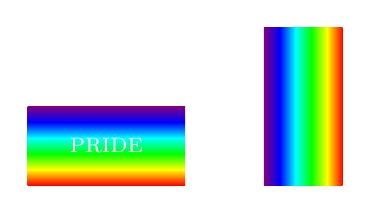
\begin{tikzpicture}[shading=rainbow]
  \shade (0,0) rectangle node[white] {\textsc{pride}} (2,1);
  \shade[shading angle=90] (3,0) rectangle +(1,2);
\end{tikzpicture}
\end{codeexample}

  Note that rainbow shadings are \emph{way} to colorful in almost all
  applications. 
\end{command}
